\documentclass{beamer}
\setbeamertemplate{navigation symbols}{}
\setbeamertemplate{bibliography item}[text]

\usepackage{beamerthemeshadow}
\usepackage{amsmath}
\usepackage{amssymb}
\usepackage{graphicx}
\graphicspath{ {./images/} }
\begin{document}
\title{Supporting Hyperplane Theorem}  
\author{Coman Florin-Alexandru}

\begin{frame}
\titlepage
\end{frame}

\begin{frame}\frametitle{Table of contents}\tableofcontents
\end{frame}

\section{Hyperplanes}
\subsection{Introduction}
\begin{frame}\frametitle{Hyperplanes}
\begin{block}{Introduction}
Hyperplanes dominate the entire theory of optimization; appearing in Lagrange multipliers, duality theory, gradient calculations, etc. The most natural definition for a hyperplane is the generalization of a plane in $\mathbb{R}^3.$
\end{block}
\end{frame}

\subsection{Definition}
\begin{frame}\frametitle{Hyperplanes}
\begin{block}{Linear variety}
A set $V$ in $\mathbb{R}^n$ is said to be \textbf{linear variety}, if, given any $x_1, x_2 \in V$, we have $\alpha x_1 + (1 - \alpha) x_2 \in V, \forall \alpha \in \mathbb{R}.$ \\
The only difference between a linear variety and a convex set is that a linear variety is the entire line passing through any two points, rather than a simple line segment.
\end{block}
\begin{block}{Definition - Hyperplane}
A \textbf{hyperplane} in $\mathbb{R}^n$ is an $(n-1)$-dimensional linear variety. It can be regarded as the largest linear variety in a space other than the entire space itself.
\end{block}
\end{frame}

\subsection{Properties}
\begin{frame}\frametitle{Hyperplanes}
\begin{block}{Proposition 1.1}
Let $a \in \mathbb{R}^n, a \neq \mathit{\Theta}$ and $b \in \mathbb{R}$. The set \\
\centerline{$H = \lbrace x \in \mathbb{R}^n : a^T x = b \rbrace$}
is a \textit{hyperplane} in $\mathbb{R}^n.$
\end{block}
\begin{block}{Proof}
Let $x_1 \in H$. Translate $H$ by $-x_1$, we obtain the set\\
\centerline{$M = H - x_1 = \lbrace y \in \mathbb{R}^n : \exists x \in H \ni y = x - x_1 \rbrace,$}
which is a linear subspace of $\mathbb{R}^n$. $M = \lbrace y \in \mathbb{R}^n : a^T y = 0 \rbrace$ is also the set of all orthogonal vectors to $a \in \mathbb{R}^n$, which is clearly $(n - 1)$ dimensional.
\end{block}
\end{frame}

\begin{frame}\frametitle{Hyperplanes}
\begin{block}{Proposition 1.2}
Let $x_1 \in H$ be an hyperplane in $\mathbb{R}^n$. Then, $\exists a \in \mathbb{R}^n \ni H = \lbrace x \in \mathbb{R} : a^T x = b \rbrace$.
\end{block}
\begin{block}{Proof}
Let $x_1 \in H$, and translate $-x_1$ obtaining $M = H - x_1$. Since $H$ is a hyperplane, $M$ is an $(n - 1)$ dimensional space. Let $a$ be any orthogonal to $M$, i.e. $a \in M^\bot$. Thus, $M = \lbrace y \in \mathbb{R}^n : a^T y = 0 \rbrace$. Let $b = a^T x_1$; we see that if $x_2 \in H, x_2 - x_1 \in M$ and therefore $a^T x_2 - a^T x_1 = 0 \Rightarrow a^T x_2 = b$. Hence, $H \subset x \in \mathbb{R} : a^T x = b$. Since $H$ is, by definition, of $(n - 1)$ dimension, and $\lbrace x\in \mathbb{R} : a^T x = b \rbrace$ is of dimension $(n - 1)$ by the above proposition, these two sets must be equal.
\end{block}
\end{frame}


\section{Half Space}
\subsection{Definition}
\begin{frame}{Half Space}
\begin{block}{Definition}
Let $a \in \mathbb{R}^n, b \in \mathbb{R}$. Corresponding to the hyperplane $H = \lbrace x : a^T x = b \rbrace$, there are \textbf{positive} and \textbf{negative closed half spaces}:
\centerline{$H_+ = \lbrace x : a^T x \geq b \rbrace, H_- = \lbrace x : a^T x \leq b \rbrace$}
and
\centerline{$\dot{H}_+ = \lbrace x : a^T x > b \rbrace, \dot{H}_- = \lbrace x : a^T x < b \rbrace.$}
Half spaces are convex sets and $H_+ \bigcup H_- = \mathbb{R}^n.$
\end{block}
\end{frame}


\section{Separating Hyperplane}
\subsection{Theorem}
\begin{frame}{Separating Hyperplane Theorem}
\begin{block}{Separating Hyperplane Theorem}
Let $X$ be a convex set and $y$ be a point exterior to the closure of $X$. Then, there exists a vector $a \in \mathbb{R}^n \ni a^T y < inf_{x \in X} a^T x$. \\
(Geometrically, a given point $y$ outside $X$, a \textbf{separating} hyperplane can be passed through the point $y$ that does not touch $X$).
\end{block}
\begin{figure}[h]
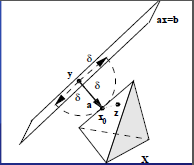
\includegraphics[width=4cm]{picture1}
\end{figure}
\end{frame}

\subsection{Proof}
\begin{frame}{Separating Hyperplane Theorem}
\begin{block}{Proof (I) \cite{1}}
Let $\delta = inf_{x \in X} |x - y| > 0.$ \\
Then, there is an $x_0$ on the boundary of $X$ such that $|x_0 - y| = \delta.$ \\
Let $z \in X$. Then, $\forall \alpha, 0 \leq \alpha \leq 1, x_0 + \alpha (z - x_0)$ is the line segment between $x_0$ and $z$. \\ 
Thus, by definition of $x_0$, $|x_0 + \alpha (z - x_0) - y|^2 \geq |x_0 - y|^2 \Leftrightarrow$ \\
$(x_0 - y)^T (x_0 - y) + 2 \alpha (x_0 - y)^T (z - x_0) + \alpha^2 (z - x_0)^T (z - x_0) \geq (x_0 - y)^T (x_0 - y) \Leftrightarrow$ \\
$2 \alpha (x_0 - y)^T (z - x_0) + \alpha^2 |z - x_0|^2 \geq 0$ \\
Let $\alpha \to 0^+$, then $\alpha^2$ tends to 0 more rapidly than $2 \alpha$. \\
\end{block}
\end{frame}

\begin{frame}{Separating Hyperplane Theorem}
\begin{block}{Proof (II)}
Thus, $(x_0 - y)^T (z - x_0) \geq 0 \Leftrightarrow$ \\
$(x_0 - y)^T z - (x_0 - y)^T x_0 \geq 0 \Leftrightarrow$ \\
$(x_0 - y)^T z \geq (x_0 - y)^T x_0 = (x_0 - y)^T y + (x_0 + y)^T (x_0 - y) = (x_0 - y)^T y + \delta^2 \Leftrightarrow$ \\
$(x_0 - y)^T y < (x_0 - y)^T x_0 \geq (x_0 -y)^T z, \forall z \in X$ (Since $\delta > 0$). \\
Let $a = (x_0 - y)$, then \\
$a^T y < a^T x_0 = inf_{z \in X} a^T z.$
\begin{flushright}$\square$\end{flushright}
\end{block}
\end{frame}


\section{Supporting Hyperplane}
\subsection{Thorem}
\begin{frame}{Supporting Hyperplane Theorem}
\begin{block}{Supporting Hyperplane Theorem}
Let $X$ be a convex set, and let $y$ be a boundary point of $X$. Then, there is a hyperplane containing $y$ and containing $X$ in one of its closed half spaces.
\end{block}
\end{frame}

\subsection{Proof}
\begin{frame}{Supporting Hyperplane Theorem}
\begin{block}{Proof \cite{1}}
Let $\lbrace y_k \rbrace$ be sequence of vectors, exterior to the closure of $X$, converging to $y$. \\
Let $\lbrace a_k \rbrace$ be a sequence of corresponding vectors constructed according to the previous theorem, normalized so that $|a_k| = 1$, such that $a_k^T y_k < inf_{x \in X}.$ \\
Since $\lbrace a_k \rbrace$ is a boundary sequence, it converges to $a$. \\
For this vector, we have $a^T y = lim a_k^T y_k \leq a x.$
\begin{flushright}$\square$\end{flushright}
\end{block}
\end{frame}

\subsection{Definition}
\begin{frame}{Supporting Hyperplane Theorem}
\begin{block}{Definition} 
A hyperplane containing a convex set $X$ in one of its closed half spaces and containing a boundary point of $X$ is said to be \textbf{supporting hyperplane} of $X$.
\end{block}
\end{frame}

\section{Bibliography}
\begin{frame}[allowframebreaks]
\frametitle{Bibliography}
    \tiny{\bibliographystyle{abbrv} }
    \bibliography{main}
\end{frame}

\end{document}
